Qubit gates and their fidelities.

\begin{parts}
	\part Density operator: $\hat{\rho} = \sum_{n} P_n \ket{\psi_n}\bra{\psi_n}$
	
	Therefore we have density matrix:
	\begin{align*}
		\rho &= \ket{\psi}\bra{\psi} \\
		&= \begin{pmatrix}
			\alpha \\ \beta
		\end{pmatrix}
		\begin{pmatrix}
			\alpha^* & \beta^*
		\end{pmatrix} \mtext{ for $\ket{\psi} = \alpha\ket{0} + \beta\ket{1}$} \\
		&= \begin{pmatrix}
			|\alpha|^2 & \alpha\beta^* \\
			\alpha^*\beta & |\beta|^2
		\end{pmatrix}
	\end{align*}
	
	Conjugate of $\rho$:
	\begin{align*}
		\rho^\dag &= \rbracket{\ket{\psi}\bra{\psi}}^\dag \\
		&= \rbracket{\bra{\psi}}^\dag \rbracket{\ket{\psi}}^\dag \\
		&= \ket{\psi}\bra{\psi} = \rho
	\end{align*}
	Thus $\rho$ is Hermitian.
	
	Also $\rho^2 = \ket{\psi}\braket{\psi | \psi}\bra{\psi} = \rho \Rightarrow \textnormal{tr}(\rho^2) = \textnormal{tr}(\rho) = 1$.
	
	In this case $\rho$ is unitary, however for a mixed state $\rho^2 \neq \rho$ hence this is not general.
	
	\part We make definition $\mathtt{TRANSPOSE} \equiv T$ for ease of writing.
	
	Then we have:
	\begin{align*}
		T\rho &= \rho^T \\
		&= \begin{pmatrix}
			|\alpha|^2 & \alpha^*\beta \\
			\alpha\beta^* & |\beta|^2
		\end{pmatrix} \\
		&= \begin{pmatrix}
			\alpha^* \\ \beta^*
		\end{pmatrix}
		\begin{pmatrix}
			\alpha & \beta
		\end{pmatrix} \\
		&= \ket{\psi^T}\bra{\psi^T}
	\end{align*}
	So $\ket{\psi^T}$ has its amplitudes in computational basis conjugated from $\ket{\psi}$.
	
	For state on z-axis, we pick $\ket{\psi} = \ket{0}$.
	
	For y-axis, we pick $\ket{\psi} = \ket{+} = (\ket{0} + \ket{1})/\sqrt{2}$.
	
	For x-axis, we pick $\ket{\psi} = \ket{R} = (\ket{0} + \mathrm{e}^{i\pi/2}\ket{1})/\sqrt{2}$.
	
	\begin{center}
		\begin{tabular}{|c|c|}
			\hline
			$\ket{\psi}$ & $\ket{\psi^T}$ \\
			\hline
			$\begin{pmatrix}
				1 \\ 0
			\end{pmatrix}$ &
			$\begin{pmatrix}
				1 \\ 0
			\end{pmatrix}$ \\
			$\begin{pmatrix}
				\dfrac{1}{\sqrt{2}} \\[1em] \dfrac{1}{\sqrt{2}}
			\end{pmatrix}$ &
			$\begin{pmatrix}
				\dfrac{1}{\sqrt{2}} \\[1em] \dfrac{1}{\sqrt{2}}
			\end{pmatrix}$ \\
			$\begin{pmatrix}
				\dfrac{1}{\sqrt{2}} \\[1em] \dfrac{i}{\sqrt{2}}
			\end{pmatrix}$ &
			$\begin{pmatrix}
				\dfrac{1}{\sqrt{2}} \\[1em] -\dfrac{i}{\sqrt{2}}
			\end{pmatrix}$ \\
			\hline
		\end{tabular}
	\end{center}
	
	For $T \sim \mathds{1}$, we have $\mathds{1}\ket{\psi} = \ket{\psi}$ for all basis, thus:
	\begin{equation*}
		\mathcal{F} =
		\begin{cases}
			1 \mtext{for z, x} \\
			\abs{\begin{pmatrix}
				\dfrac{1}{\sqrt{2}} & \dfrac{i}{\sqrt{2}}
			\end{pmatrix}
			\begin{pmatrix}
				\dfrac{1}{\sqrt{2}} \\[1em] \dfrac{i}{\sqrt{2}}
			\end{pmatrix}
			}^2 = 0
		\end{cases}
	\end{equation*}
	So average $\mathcal{F} = \diagfrac{2}{3} + 0 = \diagfrac{2}{3}$.
	
	For $T \sim \mathrm{X}$, we have:
	\begin{align*}
		\begin{pmatrix}
			1 \\ 0
		\end{pmatrix} &\rightarrow
		\begin{pmatrix}
			0 \\ 1
		\end{pmatrix} \\
		\begin{pmatrix}
			\dfrac{1}{\sqrt{2}} \\[1em] \dfrac{1}{\sqrt{2}}
		\end{pmatrix} &\rightarrow
		\begin{pmatrix}
			\dfrac{1}{\sqrt{2}} \\[1em] \dfrac{1}{\sqrt{2}}
		\end{pmatrix} \\
		\begin{pmatrix}
			\dfrac{1}{\sqrt{2}} \\[1em] \dfrac{i}{\sqrt{2}}
		\end{pmatrix} &\rightarrow
		\begin{pmatrix}
			\dfrac{i}{\sqrt{2}} \\[1em] \dfrac{1}{\sqrt{2}}
		\end{pmatrix}
	\end{align*}
	
	Hence we have:
	\begin{align*}
		\mathcal{F}\rbracket{\bra{\psi^T},\, \mathrm{X}\ket{\psi}} &= \frac{1}{3}\sbracket{
		\abs{\begin{pmatrix}
			1 & 0
		\end{pmatrix}
		\begin{pmatrix}
			0 \\ 1
		\end{pmatrix}}^2 +
		\abs{\begin{pmatrix}
			\dfrac{1}{\sqrt{2}} & \dfrac{1}{\sqrt{2}}
		\end{pmatrix}
		\begin{pmatrix}
			\dfrac{1}{\sqrt{2}} \\[1em] \dfrac{1}{\sqrt{2}}
		\end{pmatrix}}^2 +
		\abs{\begin{pmatrix}
			\dfrac{1}{\sqrt{2}} & \dfrac{i}{\sqrt{2}}
		\end{pmatrix}
		\begin{pmatrix}
			\dfrac{i}{\sqrt{2}} \\[1em] \dfrac{1}{\sqrt{2}}
		\end{pmatrix}}^2
		} \\
		&= \frac{2}{3}
	\end{align*}
	
	For $T \sim \mathtt{MEASUREMENT}$, we have:
	\begin{align*}
		\begin{pmatrix}
			1 \\ 0
		\end{pmatrix} &\rightarrow
		\begin{pmatrix}
			1 \\ 0
		\end{pmatrix} \\
		\begin{pmatrix}
			\dfrac{1}{\sqrt{2}} \\[1em] \dfrac{1}{\sqrt{2}}
		\end{pmatrix} &\rightarrow
		\begin{pmatrix}
			\dfrac{1}{2} & \\[1em] & \dfrac{1}{2}
		\end{pmatrix} \\
		\begin{pmatrix}
			\dfrac{1}{\sqrt{2}} \\[1em] \dfrac{i}{\sqrt{2}}
		\end{pmatrix} &\rightarrow
		\begin{pmatrix}
			\dfrac{1}{2} & \\[1em] & \dfrac{1}{2}
		\end{pmatrix}
	\end{align*}
	
	So we have $\mathcal{F}_z = 1$, $\mathcal{F}_x = \mathcal{F}_y =
	\begin{pmatrix}
	\frac{1}{\sqrt{2}} & \frac{1}{\sqrt{2}}
	\end{pmatrix}
	\begin{pmatrix}
		\frac{1}{2} & \\ & \frac{1}{2}
	\end{pmatrix}
	\begin{pmatrix}
		\frac{1}{\sqrt{2}} \\ \frac{1}{\sqrt{2}}
	\end{pmatrix}$.
	
	Thus average $\mathcal{F} = \diagfrac{1}{3} + \diagfrac{2}{3} \times \diagfrac{1}{2} = \diagfrac{2}{3}$.
	
	For $\mathds{1}$, since conjugation relates to the azimuthal inversion, the set of kets that satisfies $\mathcal{F} = 1$ would be the ones wiht azimuthal angle $\phi = 0$.
	
	For $\mathrm{X}$, it would be the ones with $\phi = \pm\pi/2$.
	
	For $\mathtt{MEASUREMENT}$, it would be the basis $\ket{0}$ and $\ket{1}$.
	
	\begin{figure}[H]
		\centering
		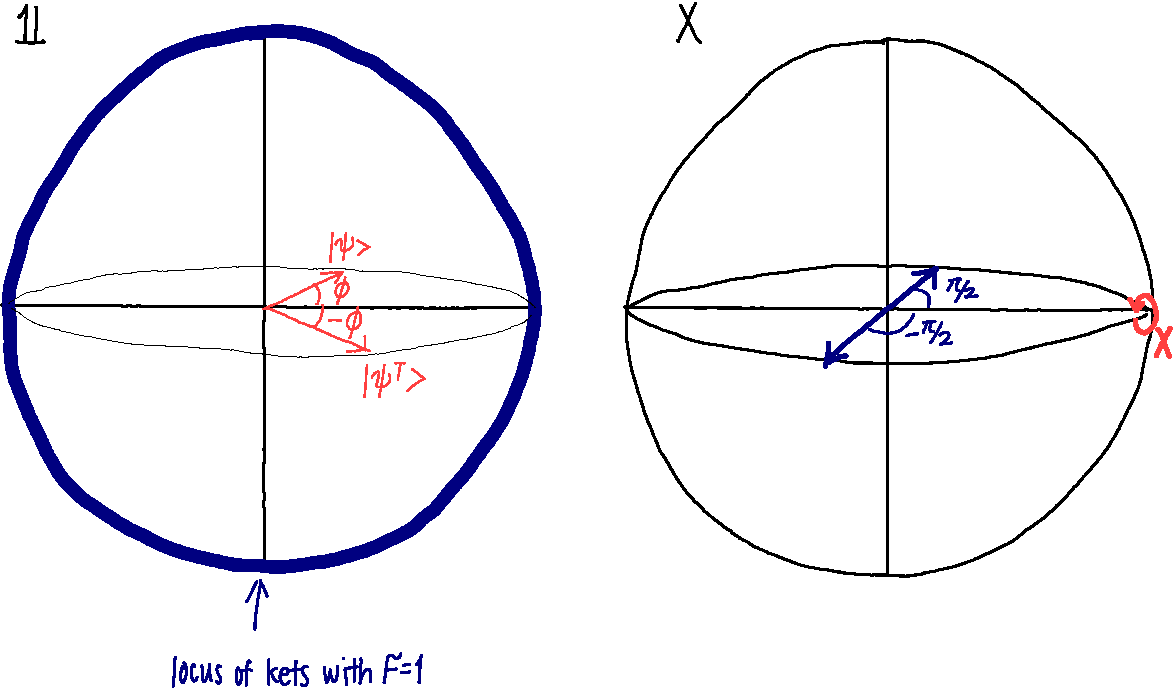
\includegraphics[width=.9\linewidth]{q5-f1}
	\end{figure}
\end{parts}